\chapter{Обзор литературы} \label{ch:ch1}
\section{Приложения квантовой информатики} \label{sec:ch1/sec1}

Метод квантового распределения ключа является одним из наиболее развитых на сегодняшний день практическим приложением квантовой информатики - области знаний на стыке фотоники, теории информации и квантовой физики, которая использует квантовые биты (кубиты), то есть квантовые системы, способные находиться в двух состояниях, для осуществления передачи, хранения и обработки информации [1]. Системы квантовой коммуникации позволяют их пользователям осуществлять рассылку симметричных криптографических ключей таким образом, что любые попытки вторжения нелегитимного пользователя в канал связи принципиально обнаруживаются. К другим перспективным приложениям квантовой информатики относятся квантовый компьютер - гипотетическое вычислительное устройство, работающее на принципах квантовой механики [2] и квантовая телепортация - передача квантового состояния на расстояние [3].


В последние годы отмечается рост интереса к прикладным аспектам квантовой информатики. В частности, основными фаворитами на получение Нобелевской премии 2012 года являлись работы по открытию и экспериментальному подтверждению квантовой телепортации под авторством основоположников квантовой криптографии Ч. Беннета и Ж. Брассара [4].  


Наибольшие прикладные успехи были достигнуты именно в системах квантовой коммуникации. В последние годы успехи в разработке экспериментальных образцов этих систем сопровождаются повышением интереса к их интегрированию в волоконно-оптические линии связи, что является необходимым условием для их широкого распространения этой технологии. В мире также появились первые коммерческие образцы [5], имеется большое количество патентов на разработки в данной сфере [6,7].


На сегодняшний день исследования в области квантовой рассылки ключа находятся в экспериментальной фазе: ранее были заложены основные принципы функционирования систем, предложен ряд способов генерации и обработки квантовых состояний, разработаны протоколы генерации ключа. Сегодня разработки ведутся с целью повышения технических характеристик систем: увеличения скорости и дальности распределения ключа, повышение спектральной эффективности, уменьшения воздействия шумов и факторов внешней среды, а также их интеграции в существующие линии связи телекоммуникационного стандарта. 

%%%%%%%%%%%%%%%%%%%%%%%%%%%%%%%%%%%%%%%%%%%%%%%%%%%%%%%%%%%%%%%%%%%%%%%%%%%%%%%%%%%%%%%%%%%%%%%%%%%%%%%%%%%%%%%%%%

\section{Системы квантовой коммуникации} \label{sec:ch1/sec2}

В современном мире требования к защите передаваемой  информации становятся все более жесткими в связи двумя проблемами:
\begin{enumerate}
	\item Условная стойкость математических алгоритмов шифрования.
Считается, что для взлома современных алгоритмов шифрования, злоумышленник не обладает достаточными вычислительными мощностями [8].
	\item Возможность появления квантового компьютера, обладающего необходимой вычислительной мощностью, чтобы в разумные сроки расшифровать закодированную информацию [9].
\end{enumerate} 


Наиболее выигрышную позицию в обозначенном выше вопросе занимает <<метод одноразового блокнота>>, предложенный Ж. Вернамом [10]. Идея этого метода заключается в обмене между легитимными пользователями секретными ключами, каждый из которых используется для шифрования только одного сообщения,  затем уничтожается. Для обеспечения безусловной стойкости применяют так называемый <<абсолютно стойкий ключ>> (АСК) [11], удовлетворяющий определенным требованиям:

\begin{enumerate}
	\item Ключ используется лишь один раз
	\item Длина ключа должна быть не менее длины шифруемого сообщения
	\item Ключ абсолютно случаен
	\item Ключ известен только легитимным пользователям
\end{enumerate}


В этих требованиях заложена проблема распространения АСК между доверенными лицами. И эту проблему можно решить, полагаясь на фундаментальные законы физики.


Итак, квантовая рассылка ключа (КРК) - направление в квантовой информатике, решающее проблему распределения <<абсолютно стойкого ключа>> между двумя и более легитимными пользователями [12].


Уникальность этого направления заключается в том, что секретность достигается за счет фундаментальных законов квантовой механики [12, 13]. Не существует способов измерения, усиления, копирования или разделения одних параметров системы без изменения других [14]. Таким образом, на основе анализа статистики принятых отсчётов можно утверждать об отсутствии или наличии в канале связи подслушивания, неизбежно влияющего на всю систему.


Принципиальная схема системы квантовой рассылки ключа (рис.\ref{fig:Fig_1}) включает в себя передатчик, именуемый Бобом (Bob), приёмник, именуемый Алисой (Alice), два связывающих их канала: квантовый и открытый. Также традиционно имеется нелегитимный пользователь (подслушиватель) - Ева (Eve) [12].


Принципиальная схема представлена на рис. \ref{fig:Fig_1}
 \begin{figure}[ht]
  \centering
  \includegraphics {Basic_scheme.pdf}
  \caption{Принципиальная схема системы квантовой рассылки ключа [12]}
  \label{fig:Fig_1}
\end{figure}


По квантовому каналу, в качестве которого используется оптоволокно, происходит распределение ключа с использованием одиночных фотонов. Открытый же канал является незащищённым и используется для выяснения легитимными пользователями изменений статистики отсчетов и коррекции ошибок в первичном ключе, переданном по квантовому каналу связи [13].

%%%%%%%%%%%%%%%%%%%%%%%%%%%%%%%%%%%%%%%%%%%%%%%%%%%%%%%%%%%%%%%%%%%%%%%%%%%%%%%%%%%%%%%%%%%%%%%%%%%%%%%%%%%%%%%%%%

\section{Протоколы квантовой коммуникации} \label{sec:ch1/sec3}

Протоколом называется алгоритм формирование квантовых кодирующих последовательностей, то есть скоррелированных наборов бит у блоков отправителя и получателя с применением квантов света. "Классическими"  считаются протоколы BB84 и B92, разработанные основоположниками направления квантовой рассылки ключа. В основе первого лежит кодирование информации о ключе в 4 состояния, в качестве которых используются, например, поляризационные степени свободы, по два в каждом из двух базисов - вертикально-горизонтальном и диагональном [12]. Второго - кодирование в 2 состояния, ортогональных друг другу, в качестве которых традиционно используется фазы сигналов. Один из методов формирования кубитов - фазовое кодирование с использованием интерферометра Маха-Цендера [13]. Данный протокол реализуется следующим образом: на первом шаге Алиса случайным образом модулирует фазу светового импульса, выбирая сдвиг фазы, равный 0 или $\pi$. (При этом Алиса и Боб заранее договариваются, какие значения фазы будут соответствовать 0 и 1 в формируемой последовательности.) Боб независимо от Алисы случайным образом модулирует фазу идентичного светового импульса, выбирая сдвиг фазы, равный 0 или π и детектирует результат интерференции этих импульсов. Если интерференция конструктивна, то Боб верно угадал фазу (в нашем рассмотрении мы не учитываем влияние шумов), и полученный бит интерпретируется как 0 или 1 в зависимости от начальной договоренности. Если интерференция деструктивна (и анализатор Боба не детектирует импульс), то возможно два случая: или Боб неверно угадал фазу, заданную Алисой, или в этот временной отсчет не было послано ни одного фотона. Процесс повторяется снова для каждого импульса. По завершению передачи Боб сообщает Алисе, в какие промежутки времени он детектировал фотоны, не сообщая, какую модуляцию он использовал. Состояния, в которых Боб не детектировал импульсы, отбрасываются.


\begin{table} [htbp]
	\centering
	\caption{Пример формирования ключа по протоколу B92.}
	\label{tab:protocol}
	\begin{tabular}{| c | c | c | c | c |}
	 \hline	Алиса                              & \multicolumn{2}{|c|}{0}   & \multicolumn{2}{|c|}{1}   \\ \hline
	  Фаза Алисы					     	   & \multicolumn{2}{|c|}{0}   & \multicolumn{2}{|c|}{1}   \\ \hline
	  \makecell{Боб выбирает \\ фазу}	    	   & 0      	                   & 180    & 0 	& 180      \\ \hline
	  \makecell{Боб детектирует \\ фотон}      & ДА                        & НЕТ    & НЕТ   & ДА       \\ \hline
	  \makecell{Алиса и Боб \\ разделяют бит}  & ДА                        & НЕТ    & НЕТ   & ДА       \\ \hline
	\end{tabular}%
\end{table}


Простейшая схема B92 (модификация интерферометра Маха-Цендера, каждое из плеч которого находится у одного из участников) представлена на рисунке \ref{fig:Fig_2}.
 

 \begin{figure}[ht]
  \centering
  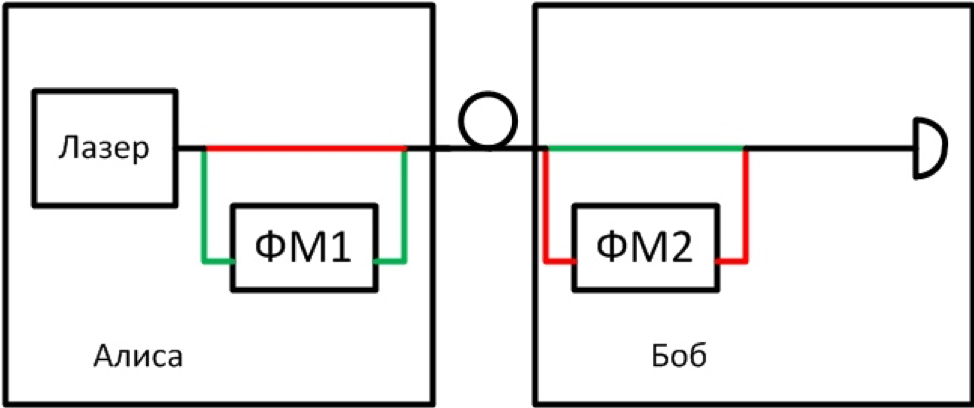
\includegraphics {Fig_2.png}
  \caption{Принципиальная схема системы квантовой коммуникации с фазовым кодированием [13]}
  \label{fig:Fig_2}
\end{figure}

Испущенный лазером импульс разделяется Алисой на две части: одна идет по "короткому" пути (красный1) и проходит через модулятор фазы (ФМ1), а второй по "длинному" пути (зеленый1). Информация кодируется изменением фазы в ФM1. После прохождения по линиям связи, импульсы приходят в такой же интерферометр на стороне Боба, где снова разделяются, формируя три вида импульсов. Первый, прошедший дважды по "короткому" пути (зеленый 2) и последний, дважды прошедший по "длинному" (красный 2), не несут никакой информации. Средний является результатом интерференции импульсов, прошедших пути красный1-красный2 и зеленый1-зеленый2. Чтобы детектировать полученный в результате интерференции импульс необходимо его отделить от мощного импульса красный1-зеленый2 с помощью электро-оптического затвора ЭЗ и направить на детектор одиночных фотонов ДОФ. Импульс красный1-зеленый2 впоследствии может использоваться в качестве опорного импульса, то есть сигнализировать о факте прибытия квантового импульса.

%%%%%%%%%%%%%%%%%%%%%%%%%%%%%%%%%%%%%%%%%%%%%%%%%%%%%%%%%%%%%%%%%%%%%%%%%%%%%%%%%%%%%%%%%%%%%%%%%%%%%%%%%%%%%%%%%

\section{Системы квантовой коммуникации на боковых частотах модулированного излучения} \label{sec:ch1/sec4}

Метод квантового распределения ключа на боковых (поднесущих) частотах модулированного излучения (КРКПЧ) был предложен в работе [16] и развивался в работах [17, 18]. Основными особенностями являются: простота по сравнению с указанными выше аналогами благодаря исключению влияния поляризации, а также отказу от работы по принципу интерферометра Маха-Цендера ввиду необходимости постоянного проведения достаточно сложной юстировки; высокая скорость передачи информации; возможность мультиплексирования сигнала с разделением по длине волны.

 
Генерация криптографического ключа по протоколу B92 в данной системе происходит следующим образом [19]:


 Световой пучок генерируется источником монохроматического излучения, в данном случае лазерным диодом. Излучение подвергается амплитудной или фазовой модуляции с помощью модулятора Алисы (ФМ1). В простейшем случае применяется периодическая синусоидальная модуляция. В результате модуляции в спектре сигнала появляются две боковые частоты, отстоящие от основной частоты оптического сигнала на величину частоты модулирующего радиочастотного сигнала. Для передачи квантового сигнала используются боковые частоты при выполнении условия $\mu \ll 1$ ( $\mu$ - среднее число фотонов в импульсе). Далее световой пучок ослабляется с помощью аттенюатора до уровня энергии одиночных фотонов. Мощность излучения на боковых частотах должна быть значительно ниже, чем на центральной частоте. Для того, чтобы среднее время между двумя генерируемыми фотонами не превышало один такт кодирования, регулируется индекс модуляции, зависящий от амплитуды модулирующего сигнала.  Ослабленный сигнал на центральной частоте представляет собой опорный световой пучок. Кодирование происходит благодаря внесению в модулирующий сигнал некоторого фазового сдвига. Блок отправителя соединен с блоком получателя волоконно-оптической линией связи. При достижении приёмного устройства сигнал подвергается повторной модуляции по аналогии с устройством отправителя (ФМ2). При этом в модулирующий сигнал также вносится случайный фазовый сдвиг. Мощность излучения на боковых частотах зависит от значений фазового сдвига, внесенных на передающем устройстве и приемном устройстве. Если они совпали, т.\:е. разность фаз двух модулирующих радиочастотных сигналов равна нулю ($\phi$A-$\phi$В=$0$), на боковых частотах наблюдается конструктивная интерференция, и мощность оптического сигнала отлична от нуля. В случае, когда модулирующие радиочастотные сигналы Алисы и Боба находятся в противофазе, т.\:е. разность фаз модулирующих сигналов равна $\pi$ ($\phi$A-$\phi$В=$\pi$), наблюдается деструктивная интерференция, и мощность сигнала на боковых частотах равняется нулю [16].
 
 
При конструктивной интерференции значениям выбранных сдвигов фаз (0 или π) соответствуют, по договоренности, биты (0 или 1). Боб по открытому каналу сообщает Алисе моменты времени, когда совпали их сдвиги фаз, и та, в свою очередь, отбрасывает лишнюю информацию. Так генерируется <<просеянный>> ключ, который подлежит процедуре коррекции ошибок. 

 \begin{figure}[ht]
  \centering
  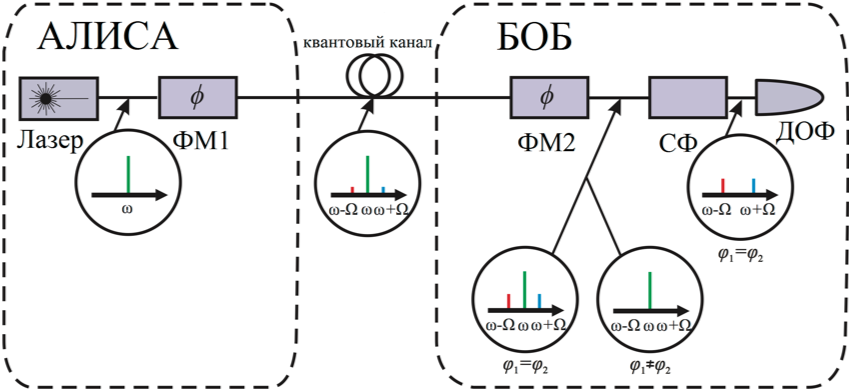
\includegraphics {Fig_3.png}
  \caption{Принципиальная схема системы квантовой коммуникации на боковых частотах модулированного излучения}
  \label{fig:Fig_3}
\end{figure}


%%%%%%%%%%%%%%%%%%%%%%%%%%%%%%%%%%%%%%%%%%%%%%%%%%%%%%%%%%%%%%%%%%%%%%%%%%%%%%%%%%%%%%%%%%%%%%%%%%%%%%%%%%%%%%%%%%

\section{Измерительное оборудование в системах квантовой коммуникации} \label{sec:ch1/sec5}


Системы квантовой коммуникации (СКК) оперируют с крайне низкоинтенсивным излучением в волоконно-оптических линиях связи (ВОЛС), где в среднем в каждом тактовом отсчете сосредоточена энергия менее одного фотона. Детекторы одиночных фотонов (ДОФ) способны улавливать подобные сигналы, что делает их неотъемлемой частью СКК. Условно ДОФ можно разделить на две группы: широкодоступные и узкоспециализированные. Очевидно, что детекторы из второй группы, например, криогенные термоэлектрические детекторы (QVD) [17] и детекторы, основанные на поглощении в холодном атомном паре [18], не могут быть использованы серийно в производстве систем СКК. Поэтому в данном разделе рассматриваются основные виды которые широко применимых ДОФ:

\begin{enumerate}
	\item на основе лавинных фотодиодов для однофотонного излучения (single-photon avalanche diode, SPAD);
	\item использующие полевой транзистор, обогащенный квантовыми точками, с оптическим затвором (quantum-dot optically gated field-effect transistor, QDOGFET);
	\item использующие сверхпроводящие нанопроволоку (superconducting nanowire single-photon detector, SNSPD);
	\item использующий джозефсоновский переход (superconducting-tunnel-junction detector, STJ);
	\item использующие сенсор, реагирующий на переход материала из сверхпроводящего состояния в проводящее (transition-edge sensor, TES);
	\item счетчик фотонов видимого света (visible-light photon counter, VLPC) и твердотельный фотоумножитель (solid-state photomultiplier, SSPM).
\end{enumerate}

На основании сравнительной характеристики будет оценена целесообразность использования данных ДОФ для СКК.

\subsection{Лавинные фотодиоды для однофотонного излучения} \label{subsec:ch1/sec5/sub1}

ДОФ этого типа используют процесс, схожий с тем, что происходит в фотоумножителе [19]. В отличие от фотоумножителя, в фотодиоде поглощение фотона рождает электрон-дырочную пару, которая порождает аналогичное увеличение числа заряженных частиц благодаря напряжению, приложенному вдоль кристаллической решетки полупроводника. Лавинные фотодиоды, используемые для ИК излучения, имеют низкие типичные показатели квантовой эффективности 10-20~\%  (доля излучения, которая успешно переведена в электрический сигнал и зарегистрирована). Они также характеризуются достаточно высокими значениями частоты темновых срабатываний (ложные срабатывания детектора в отсутствие входящего излучения, зачастую вызванного теплом окружающей среды), поэтому диод охлаждают до 210-250 К, например, термоэлектрическими охладителями. Даже в этом случае уровень темновых отсчётов для коммерческих ДОФ данного типа составляет порядка 1-10 кГц. Для лавинных детекторов характерна остаточная пульсация, когда электроны из лавины ненадолго <<застревают>>, например, в дефектах и, освобождаясь, порождают вторичные лавины. Необходимо некоторое время для выхода в штатный режим работы, поэтому у таких диодов обычно относительно высокое мертвое время (время, когда детектор сразу после срабатывания не может повторно зарегистрировать сигнал), что может ограничить тактовую частоту следования квантовых сигналов в СКК.

\subsection{ДОФ, использующий полевой транзистор, обогащенный квантовыми точками, с оптическим затвором} \label{subsec:ch1/sec5/sub2}

Совмещение полевого транзистора с оптическим затвором из квантовых точек, расположенных между стоком и истоком, позволяют добиться регистрации одиночных ИК фотонов [20]. Квантовые точки захватывают заряженные частицы, рожденные падающим светом, изменяя приложенное электрическое поле, что ведет к изменению протекающего по транзистору тока - по данному изменение и производится детектирование сигнала. Однако низкое быстродействие данного детектора не соответствует типовым системам СКК. Квантовая эффективность не превышает 15~\%, а максимальная тактовая частота следования квантовых сигналов составляет всего 50 кГц. Кроме того, для работы данного ДОФ необходимы низкие рабочие температуры (от 70 К и ниже). При этом вероятность темновых срабатываний относительно высока.

\subsection{ДОФ, использующие сверхпроводящую нанопроволоку} \label{subsec:ch1/sec5/sub3}

Данный тип ДОФ является одним из самых быстрых. Он способен регистрировать квантовые состояния с частотой следования до единиц гигагерц [21]. Основным элементом здесь служит площадка со сверхпроводящей тонкой проволокой (superconducting nanowire), запитанная током немного меньшим, чем критический, выше которого волокно выходит из сверхпроводящего режима. В таком случае поглощенный фотон оставляет небольшой участок нагретым и, соответственно, в проводящем состоянии. Поэтому ток начинает огибать этот участок с нормальной проводимостью. В результате ток превышает критическое значение, что приводит к переходу в проводящий режим всего участка вдоль ширины волокна. Появление участка с сопротивлением выражается в соответствующем скачке напряжения во внешней цепи, что и свидетельствует о детектировании фотона. Поскольку данный механизм детектирования требует очень узкой проволоки (порядка 100 нм), его складывают меандром, для создания эффективной рабочей поверхности. Для повешения эффективности детектирования, сверху волокно покрывают отражающей поверхностью, что в итоге образует резонатор, значительно улучшающий характеристики детектора. В подобных устройствах используют в основном проволоку из нитрида ниобия, однако из-за высокого коэффициента отражения у данного материала - необходимо просветляющее покрытие, благодаря которому можно добиться высокого значения квантовой эффективности до 60~\%. Ввиду того, что детектор работает в сверхпроводящем режиме, ему необходимы низкие рабочие температуры менее 4 К. В этом режиме он характеризуется низким уровнем темновых отсчётов ($10^{-2}$-$10^2$ Гц), что важно при реализации дальнодействующих СКК.

\subsection{ДОФ, использующие джозефсоновский переход} \label{subsec:ch1/sec5/sub4}

Основным элементов для данного типа детекторов служит джозефсоновский переход - две части сверхпроводника разделенных сверхтонким (порядка 1 нм) диэлектриком, см., например, [22]. Фотон, падающий на сверхпроводящую область, вызывает распад большого числа куперовских пар электронов (квазичастицы), т.\:к. его энергия в тысячи раз больше энергии связи. Свободные электроны после распада пар способны туннелировать через диэлектрик во вторую часть сверхпроводника с крайне высокой вероятностью. Поскольку рабочая температура детектора на порядок ниже переходной температуры в сверхпроводящее состояние, куперовских пар распавшихся за счет иных процессов, нежели за счет поглощенных сигнальных фотонов, значительно меньше, что позволяет однозначно зарегистрировать однофотонное излучение. Таким образом, данный вид детекторов позволяет детектировать фотоны с эффективностью, не превышающей 45~\%, частотой следования фотонов порядка десятков кГц, однако при крайне низких рабочих температурах 0,37 К.

\subsection{Детекторы одиночных фотонов, использующий сенсор, реагирующий на переход материала из сверхпроводящего состояния в проводящее} \label{subsec:ch1/sec5/sub5}

Данный сенсор работает по принципу болометра: при поглощении излучения повышается температура сенсора [23]. Для достижения чувствительности к одиночным фотонам необходима крайне малая теплоемкость поглощающего материала, и температурный сенсор должен обладать чрезвычайно высоким откликом на малое изменение температуры. Это возможно при изготовлении сенсора из тонкого сверхпроводящего материала, и его работы точно при температуре перехода из сверхпроводящего режима в обычный (порядка 100 мК) так, что небольшое изменение температуры отражается в значительном изменении сопротивления. Большей точности измерения колебаний сопротивления можно добиться, используя сверхчувствительный магнитометр, основанный на сверхпроводящем квантовом интерферометре (SQUID). Данный вид детекторов обладает самым большим показателем квантовой эффективности среди прочих - 95~\% для фотонов в ИК области. Несмотря на это, максимальная частота следования фотонов ограничена порогом в 100 кГц.

\subsection{ДОФ видимого света и твердотельный фотоумножитель} \label{subsec:ch1/sec5/sub6}

С точки зрения квантовой эффективности, данный детектор может сравниться с предыдущим, но в области видимого света, где она достигает 90~\% [24]. Принцип работы схож с лавинным диодом, но в данном случае не электрон, а дырка, выбитая падающим излучением, ускоряется к легированной части полупроводника, где уже рождает электронную лавину. Несмотря на высокое значение квантовой эффективности, остальные параметры достаточно низки: максимальная скорость детектирования фотонов составляет 100 кГц, частота темновых срабатываний велика - не менее 20 кГц. Схожими по конструкции и принципу работы являются твердотельные фотоумножители [25]. Они обладают широкой спектральной восприимчивостью, что, в свою очередь, требует экранирования от дальнего ИК излучения, которое не представляет интереса.

\subsection{Cравнительная характеристика ДОФ для СКК} \label{subsec:ch1/sec5/sub7}

Ниже представлена таблица 1, в которой представлены ключевые параметры детекторов, описанных в предыдущих разделах.

\begin{table} [htbp]
	\centering
	\caption{Сравнительные характеристики распространённых ДОФ.}
	\label{tab:SPD_compare}
	\begin{tabular}{| c | c | c | c | c |}
	
	 \hline \makecell{Тип \\детектора} & \makecell{Рабочая T,\\~K} & \makecell{Квантовая \\эффективность,\\~\%} & \makecell{Максимальная \\частота \\регистрации \\квантовых \\сигналов} & \makecell{Темновые отсчеты, \% \\(от частоты \\регистрации \\квантовых \\сигналов)}   \\ \hline
	  SPAD         & 210-250    & < 20    & 300 МГц     & < 0,1   \\ \hline
	  STJ	   	   & < 1        & > 45    & 10 кГц  	& < 0,1      \\ \hline
	  QDOGFET      & < 80       & < 15    & 50 кГц      & < 1       \\ \hline
	  TES          & < 0,1      & > 90    & 1 МГц       & < 0,01       \\ \hline
	  \makecell{VLPC\\/SSPM} & < 10      & < 90    & 100 кГц       & < ~20      \\ \hline
	  SNSPD          & < 10      & < 60    & 3 ГГц       & < 0,0001       \\ \hline
	  
	\end{tabular}
\end{table}

На основе выполненного сравнения можно сделать следующие выводы. 


Лавинные фотодиоды для однофотонного излучения (SPAD) рекомендуется использовать для СКК. Это объясняется тем, что они работают при температурах, которые возможно обеспечить без дополнительного охлаждающего криогенного оборудования, имеют оптоволоконный интерфейс и обладают максимальной частота регистрации квантовых сигналов ниже, чем предполагаемая частота смены фазы квантовых состояний электроникой СКК. Относительно низкая квантовая эффективность и высокий уровень темновых срабатываний, однако, позволяет использовать данный вид детекторов на малых и средних дистанциях при небольших потерях в линиях ВОЛС (до 10-15 дБ).


ДОФ, использующий джозефсоновский переход (STJ) не рекомендуется использовать для приложений СКК ввиду низкой максимальной частоты регистрации квантовых сигналов и крайне низких рабочих температур, обеспечение которых является сложным технологическим процессом, увеличивающим их стоимость.


ДОФ, использующий полевой транзистор, обогащенный квантовыми точками, с оптическим затвором (QDOGFET) не рекомендуется использовать для приложений СКК по причине низкой скорости срабатывания.


ДОФ, использующий сенсор, реагирующий на переход материала из сверхпроводящего состояния в проводящее (TES) не рекомендуется использовать для приложений СКК ввиду низкой максимальной частоты регистрации квантовых сигналов и крайне низких рабочих температур, обеспечение которых является сложным технологическим процессом.


Счетчик фотонов видимого света (VLPC) и твердотельный фотоумножитель (SSPM) не рекомендуется использовать для приложений СКК по причине низкой скорости срабатывания.


ДОФ, использующий сверхпроводящую нанопроволоку (SNSPD) рекомендуется использовать для приложений СКК, т.\:к. они работают при температурах жидкого гелия, что возможно обеспечить в свою очередь и компенсируется высокими ключевыми показателями, которые обеспечат штатную работу системы СКК. Данный тип детекторов следует использовать в каналах с относительно высокими потерями (от 15 дБ). 

%%%%%%%%%%%%%%%%%%%%%%%%%%%%%%%%%%%%%%%%%%%%%%%%%%%%%%%%%%%%%%%%%%%%%%%%%%%%%%%%%%%%%%%%%%%%%%%%%%%%%%%%%%%%%%%%%

\section{Атаки злоумышленника} \label{sec:ch1/sec6} 

В действительности существует значительное отличие между моделями, которые используются для теоретического подтверждения возможности формирования абсолютно стойких ключей квантовыми методами, и практическими реализациями таких систем. Во втором случае всегда существует малая вероятность того, что система или устройства будут иметь отклонение от усредненных параметров. Другим важным фактором является то, что компоненты таких систем зачастую не разрабатывались специально под данную задачу и поэтому потенциально могут иметь ряд других режимов, характеристик и свойств в других условиях и для применения в изначальных целях. Этими нюансами может воспользоваться злоумышленник, который хочет вопреки ограничениям остаться незамеченным и при этом получить максимальное количество ключевой информации. Известны ряд неидеальностей, которые, если их не учитывать, позволяют злоумышленнику добиваться значительных результатов. Такой подход и используемые для этого методы называются \textit{квантовым взломом} (quantum hacking). Это могут быть атаки злоумышленника с разделением пучка фотонов, формируемого в результате ослабления когерентного лазерного излучения, в котором статистика числа фотонов в импульсе подчиняется распределению Пуассона. Это значит, что существует ненулевая вероятность обнаружить в одном импульсе многофотонные состояния, отделить часть энергии и зафиксировать квантовое состояние, оставшись незамеченным. Другим потенциально уязвимым звеном систем квантовой коммуникации является детектор одиночных фотонов. Ниже обосновывается уязвимость систем при использовании таких устройств и возможные типы атак злоумышленника с использованием данной уязвимости. 

%	\subsection{Атака с разделением пучка фотонов}  \label{subsec:ch1/sec6/sub1}


%	\subsection{Атака типа перехват} \label{subsec:ch1/sec6/sub2}


%	\subsection{Атака типа перехват-пересылка} \label{subsec:ch1/sec6/sub3}


\subsection{Атака на детектор на основе ЛФД} \label{subsec:ch1/sec6/sub4}

Первым этапом проведения атаки с навязыванием ключа является определение возможности выведения детектора из режима счета фотонов (режима Гейгера). Известно, что вольт-амперная характеристика лавинного фотодиода имеет вид, представленный на рисунке \ref{fig:APDs_VA}.    

 \begin{figure}[ht]
  \centering
  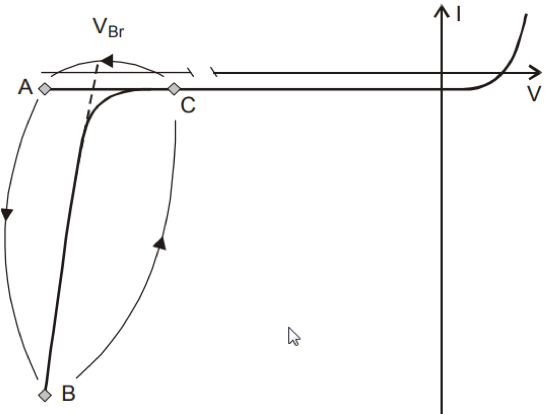
\includegraphics{APDs_VA.png}
  \caption{Вольт-амперная характеристика ЛФД}
  \label{fig:APDs_VA}
\end{figure}


Лавинный фотодиод работает при обратном напряжении смещения $-V_{bias}$ близком к напряжению пробоя $-V_{breakdown}$. Типичная величина находится в диапазоне от -40~В до -60~В. При величине обратного напряжения смещения ниже напряжения пробоя ЛФД находится в линейном режиме, где величина фототок $I_{APD}$ линейно зависит от падающей оптической мощности. При увеличении величины обратного смещения выше напряжения пробоя ЛФД переходит в режим счета фотонов, или режим Гейгера. В этом режиме даже энергии единиц фотонов достаточно для формирования лавины зарядов и резкого скачка фототока. При превышении некоторого порогового значения $I_{det}$, регулируемого уровнем срабатывания компаратора, формируется электрический импульс, который и интерпретируется, как регистрация одиночного фотона. 

 \begin{figure}[ht]
  \centering
  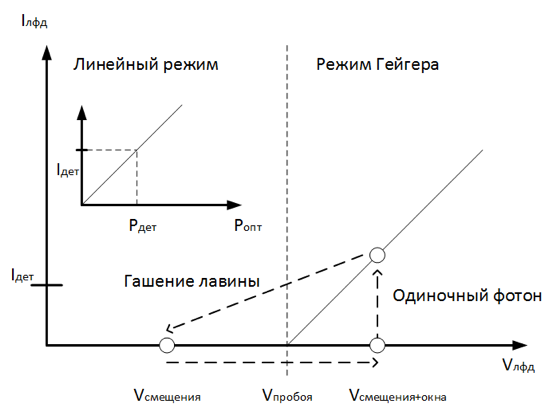
\includegraphics{Vbreakdown}
  \caption{Граница между режимами работы ЛФД при подаче обратного напряжения смещения}
  \label{fig:Vbreakdown}
\end{figure}

Гашение лавины в самом простом случае происходит благодаря последовательно подключенному в цепь резистору, как показано на рисунке \ref{fig:Quenching}. Существуют также схемы активного гашения лавины.  

 \begin{figure}[ht]
  \centering
  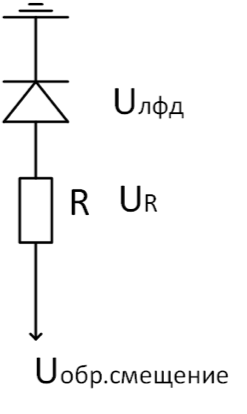
\includegraphics{Quenching}
  \caption{Принципиальная электрическая схема подключения ЛФД для регистрации одиночных фотонов}
  \label{fig:Quenching}
\end{figure}


Для снижения уровня шумов срабатываний ДОФ на базе ЛФД функционируют в режиме стробирования, когда в момент ожидаемого прибытия фотона на диод подается дополнительное напряжение в форме импульса, т.\:н. окно срабатывания $-V_{gate}$, величиной около 3~В. Благодаря этому импульсу диод переходит из линейного режима при величине напряжении $-V_{bias}$, в котором он прибывает относительно длительное время порядка единиц микросекунд, в режим счета фотонов, где $-V_{bias+gate} < - V_{breakdown}$.  

\subsection{Атака с навязыванием ключа ( Faked-state attack)} \label{subsec:ch1/sec6/sub5}


В работе показана полноценная реализация атаки с использованием уязвимости детектора на основа ЛФД. Злоумышленник имеет модифицированный приёмный узел, аналогичный блоку получателя м связанный с модифицированным узлом отправителя. Первый принимает квантовые состояния от легитимного отправителя и те случаи, где происходит совпадения посылает в модифицированный узел отправителя. Там используется интенсивное оптическое излучение для контроля детектора фотонов и формирования срабатываний в требуемых злоумышленнику отсчетах. Таким образом, он является незамеченным обладателем ключевой информации. 

 \begin{figure}[ht]
  \centering
  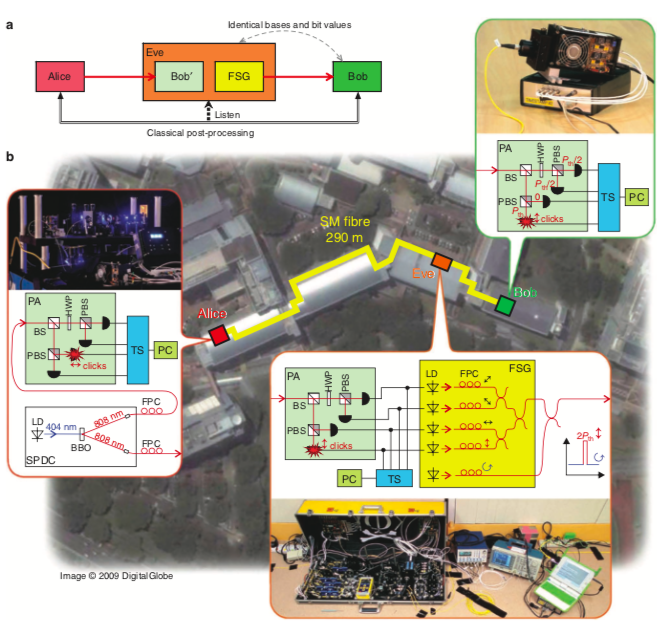
\includegraphics[scale=0.5]{FSA.png}
  \caption{Принципиальная схема проведения атаки с поддельными состояниями}
  \label{fig:FSA}
\end{figure}

\pagebreak
%%%%%%%%%%%%%%%%%%%%%%%%%%%%%%%%%%%%%%%%%%%%%%%%%%%%%%%%%%%%%%%%%%%%%%%%%%%%%%%%%
%	\subsection{Атака на SNSPD} \label{subsec:ch1/sec6/sub6}


%%%%%%%%%%%%%%%%%%%%%%%%%%%%%%%%%%%%%%%%%%%%%%%%%%%%%%%%%%%%%%%%%%%%%%%%%%%%%%%%%%%%%%%%%%%%%%%%%%%%%%%%%%%%%%%%%%

\section{Известные контрмеры против атак на измерительное оборудование} \label{sec:ch1/sec7}

Существует ряд решений для предотвращения атаки с навязыванием ключа. Ниже перечислены основные. Однако, следует отметить, что строгое доказательство секретности, а также многочисленные экспериментальные работы, подтверждающие практическую ценность есть только у предпоследнего подхода. Остальные контрмеры требуют исследования в стенах лабораторий, практикующих квантовый взлом. 

\subsection{Статистика счета фотонов} \label{subsec:ch1/sec7/sub1}

В работе предложена контрмера, основанная на наборе статистики фотонов, которые поступают на светоделитель с двумя детекторами. В случае применения атаки с <<ослеплением>> изменяется количество одновременных совпадений на этих двух детекторах относительно их нормального режима работы. 

 \begin{figure}[ht]
  \centering
  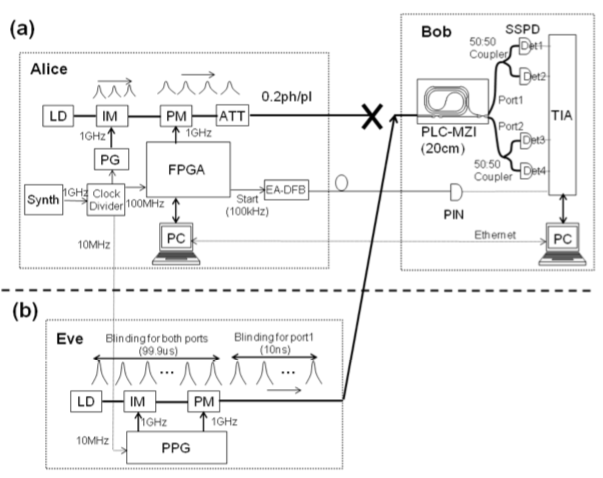
\includegraphics[scale=0.5]{PhotonStatistics.png}
  \caption{Принципиальная схема контрмер на основе статистики фотонов}
  \label{fig:PhotonStatistics}
\end{figure}

\subsection{Измерение фототока} \label{subsec:ch1/sec7/sub2}

Очевидным решением является активный мониторинг фототока, протекающего в ЛФД при попадании на него оптического излучения, и наблюдении лавинного пробоя, как показано на рисунке \ref{fig:Photocurrent}. 

 \begin{figure}[ht]
  \centering
  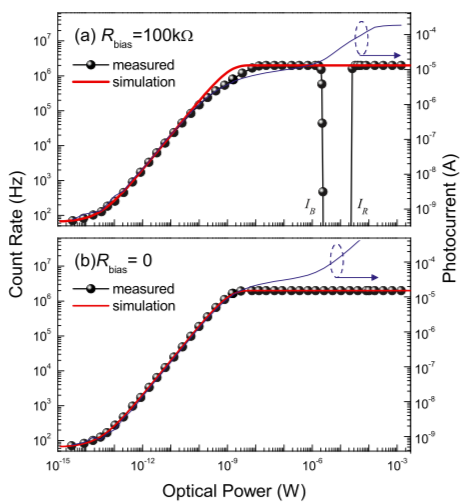
\includegraphics[scale=0.5]{Photocurrent.png}
  \caption{Зависимость количество отсчетов и фототока от интенсивности падающего излучения}
  \label{fig:Photocurrent}
\end{figure}
\pagebreak

\subsection{MDI-протокол} \label{subsec:ch1/sec7/sub3}

В работе предложен метод, в основе которого лежит предположение о том, что измерительный узел доступен злоумышленнику, который при этом знает какие из детекторов произвели срабатывание и в какой временной отсчет, однако при этом не имеют информации о том, какое квантовое состояние в блоках Алисы и Боба применялось. Это достигается за счет интерференции слабых когерентных импульсов на светоделителе внутри недоверенного узла регистрации. В процессе постселекции легитимные пользователи выявляют результат однофотонной интерференции, который привел к срабатыванию, и соотвествующие ему состояние, которые были использованы. Такой подход получил название MDI (measuerement-device-independent) и нашел широкое применение для исследований, благодаря устойчивости к атакам на измерительное оборудование. Однако, на практике ввиду чрезвычайному усложнению оптической схемы и условий, при которых наблюдается интерференция, почти не применяется в условиях близких к реальным. 


 \begin{figure}[ht]
  \centering
  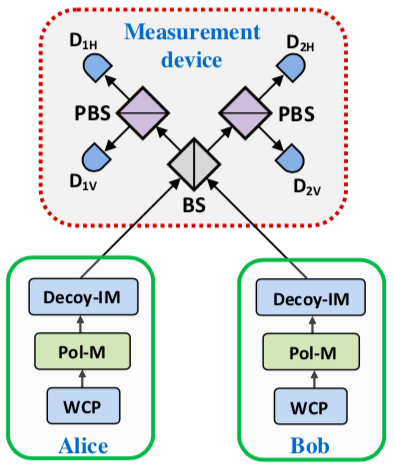
\includegraphics[scale=0.5]{MDI_scheme.png}
  \caption{Принципиальная схема системы с независимым измерительным устройством MDI}
  \label{fig:MDI_scheme}
\end{figure}


\subsection{Twin-Field протокол} \label{subsec:ch1/sec7/sub4}


Развитием темы MDI с применением фазовых состояний является протокол Twin-Field (близнецовые поля), где так же применяется анонсирование измерительным узлом, доступным злоумышленнику, результата интерференции когерентных состояний на светоделителе, которые приводят к срабатыванию детекторов одиночных фотонов. Отличительной особенностью является то, что в отличие от MDI, где для минимизации корреляции по фазе последовательности импульсов от каждого из источников, используется их рандомизация, то есть изменение фазы случайным образом, в протоколе Twin-Field используется результат интерференции когерентных состояний с определением секторов на фазовой плоскости и отбрасыванием фазовых состояний, соответствующих разным секторам в процессе постоработки.

 
 \begin{figure}[ht]
  \centering
  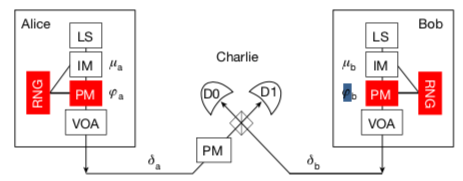
\includegraphics[scale=0.5]{TF_scheme.png}
  \caption{Принципиальная схема системы с независимым измерительным устройством}
  \label{fig:TF_scheme}
\end{figure}
%%%%%%%%%%%%%%%%%%%%%%%%%%%%%%%%%%%%%%%%%%%%%%%%%%%%%%%%%%%%%%%%%%%%%%%%%%%%%%%%%%%%%%%%%%%%%%%%%%%%%%%%%%%%%%%%%%

\section{Выбор направления исследований. Цели и задачи работы} \label{sec:ch1/sec8}

Системы квантовой коммуникации на боковых частотах модулированного излучения зарекомендовали себя, как перспективное направление коммерчески доступных устройств квантового распределения ключа с практически значимыми характеристиками мирового уровня, подтвержденными в ряде научных публикаций в международных изданиях, формализованным доказательством безусловной секретности используемого протокола, применением на нескольких полигонах, развернутых на территории Российской Федерации, совместной с ведущими компаниями в области телекоммуникационной связи, банковского сектора и региональными инжиниринговыми центрами. 


С научной и инженерной точки зрения данный класс систем имеет большой задел:

\begin{enumerate}
	\item Экспериментальная демонстрация передачи квантовых состояний на основе технологии квантовой коммуникации на боковых частотах модулированного излучения в телекоммуникационной линии связи дальностью свыше 250 км. 
	\item Разработка функциональной схемы и экспериментальная реализация оптико-электронного устройства квантовой передачи информации на боковых частотах, включающую подсистему непрерывной синхронизации модулей отправителя и получателя, подсистему компенсации неконтролируемого изменения поляризации в оптическом волокне.
	\item Экспериментально продемонстрировано спектральное уплотнение каналов на боковых частотах. 
	\item Разработка функциональной схемы и экспериментальная реализация оптико-электронного устройства квантовой передачи информации на боковых частотах, включающую подсистему непрерывной синхронизации модулей отправителя и получателя, подсистему компенсации неконтролируемого изменения поляризации в оптическом волокне.
	\item Экспериментальная демонстрация применимости данной технологии для квантового распределения ключа в открытом пространстве, а не только в волоконно-оптических линиях связи. 
\end{enumerate}


Однако, устойчивость квантовых систем передачи информации на боковых частотах к воздействию нелегитимного пользователя на измерительной оборудование ранее не была исследована. 


{\aim} данной работы является исследование возможностей злоумышленника по получению секретного ключа с использованием атак на измерительное оборудование систем квантовой коммуникации на боковых частотах и разработка методов противодействия атакам.


Для~достижения поставленной цели ставились следующие {\tasks}:
\begin{enumerate}
  \item Исследование устойчивости детектора одиночных фотонов, применяемого в системах квантовой коммуникации на боковых частотах, к атакам с выведением из режима Гейгера (<<ослеплением>>). 

  \item Оценка возможностей злоумышленника при атаке с выведением из режима Гейгера для систем квантовой коммуникации на боковых частотах. 

  \item Разработка оптической схемы системы квантовой коммуникации, устойчивой к атакам на измерительное оборудование. 

  \item Разработка протокола квантовой рассылки ключа, устойчивого к атаке на измерительное оборудование. 

\end{enumerate}
